\newpage
\section{New Baselines}
\begin{table}[htbp]
\centering
\caption{\textbf{Additional baseline comparisons.}
    This table extends the averaged comparison in~\Cref{tab:main_results_avg}
    with five newly evaluated baselines: UCE~\citep{gandikota2024unified}, RECE~\citep{gong2024reliable}, CPE~\citep{lee2025concept}, TRUST~\citep{kori2026selective}, SLD~\citep{schramowski2023safe}, and SAFREE~\citep{yoon2025safree}.
    Methods are grouped by intervention type: closed-form, fine-tuning,
    or inference-time. Cells report mean $\pm$ standard deviation across
    the evaluated target concepts, using the same erasure and retention
    metrics as the main table. The \emph{Original} row denotes the
    unedited-model reference for this comparison.}
\resizebox{\textwidth}{!}{%
\begin{tabular}{llcccccc}
\toprule
& & \multicolumn{2}{c}{\textbf{Erasure}} & \multicolumn{3}{c}{\textbf{Retention}} & \\
\cmidrule(lr){3-4} \cmidrule(lr){5-7}
\textbf{Method} & \textbf{Type} & UA$\uparrow$ & IRR$\downarrow$ & IRA$\uparrow$ & NP$\uparrow$ & CP$\uparrow$ & DamageGap$\downarrow$ \\
\midrule
uCE    & Closed-form & $80.6 \pm 18.4$ & $10.5 \pm 23.4$ & $67.1 \pm 12.4$ & $88.6 \pm 25.1$ & $99.3 \pm 3.1$  & $10.7 \pm 25.4$ \\
RECE   & Closed-form & $99.4 \pm 0.9$  & $3.0 \pm 4.0$   & $43.3 \pm 12.1$ & $56.1 \pm 10.6$  & $93.5 \pm 2.0$  & $37.4 \pm 10.2$ \\
\midrule
CPE    & FT          & $99.6 \pm 0.9$  & $4.7 \pm 9.4$   & $53.4 \pm 12.4$ & $71.9 \pm 18.1$  & $99.6 \pm 2.6$ & $18.7 \pm 19.3$ \\
TRUST    & FT          & $94.2 \pm 2.2$  & $6.5 \pm 3.5$   & $53.2 \pm 13.7$ & $76.4 \pm 9.1$  & $98.0 \pm 5.0$ & $11.6 \pm 12.2$ \\
\midrule
SLD    & Inf. & $99.6 \pm 0.9$  & $0.5 \pm 0.9$   & $35.0 \pm 8.1$  & $58.8 \pm 16.8$  & $89.1 \pm 4.1$  & $30.3 \pm 16.3$ \\
SAFREE & Inf. & $91.4 \pm 11.4$ & $8.4 \pm 10.2$  & $39.9 \pm 8.6$  & $64.7 \pm 16.0$  & $85.7 \pm 12.2$ & $21.0 \pm 19.4$ \\
\bottomrule
\end{tabular}%
    }
    \label{tab:additional_baselines}
\end{table}

\begin{figure}[htbp]
\centering
\begin{minipage}[c]{0.45\linewidth}
\centering
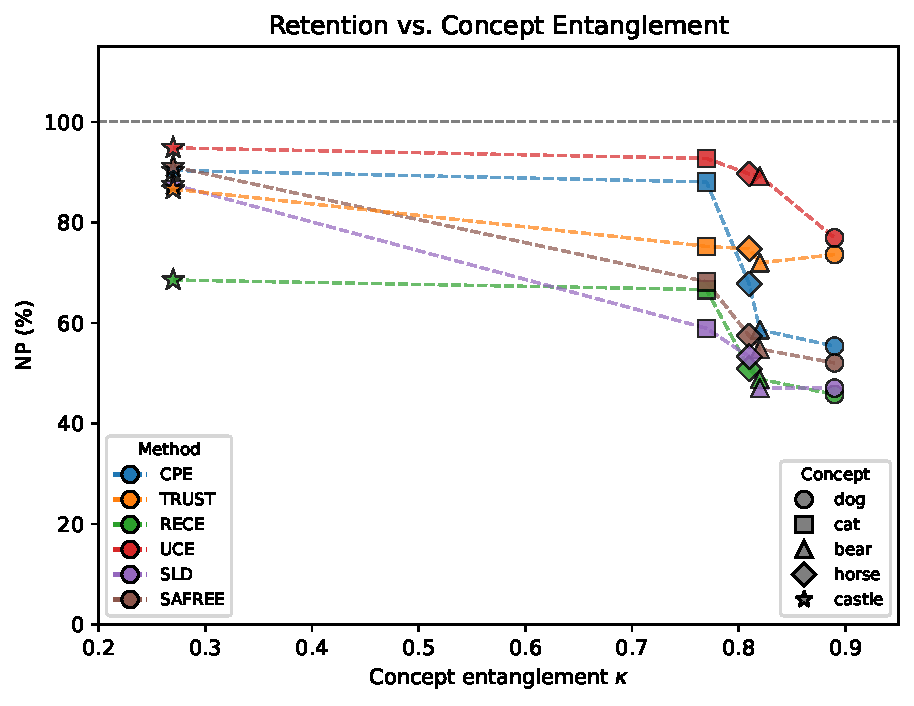
\includegraphics[width=\linewidth]{img/pareto_new_baselines_ua_only.pdf}
\end{minipage}\hfill
\begin{minipage}[c]{0.45\linewidth}
\centering
\scriptsize
\setlength{\tabcolsep}{5pt}
\begin{tabular}{lccc}
\toprule
\textbf{Concept} & $\hat\kappa$ & NP$\uparrow$ & IRA-ratio$\uparrow$ \\
\midrule
\texttt{castle} & 0.27 & 86.47 & 0.79 \\
\texttt{cat}    & 0.77 & 74.88 & 0.78 \\
\texttt{horse}  & 0.81 & 62.54 & 0.74 \\
\texttt{bear}   & 0.82 & 59.71 & 0.70 \\
\texttt{dog}    & 0.89 & 56.58 & 0.65 \\
\midrule
\multicolumn{2}{l}{Spearman $\rho$} & $-1.0$ & $-1.0$ \\
\bottomrule
\end{tabular}
\end{minipage}
\caption{\textbf{Neighbor preservation scales inversely with $\hat\kappa$.} \emph{Left:} NP for each (method, concept) pair. \emph{Right:} New baseline's NP and in-domain retention ratio across the five concepts (Spearman $\rho = -1.0$ for both).}
\label{fig:kappa_np_scaling_new}
\label{tab:kappa_scaling_new}
\vspace{-2mm}
\end{figure}


\begin{figure}[htbp]
    \centering
    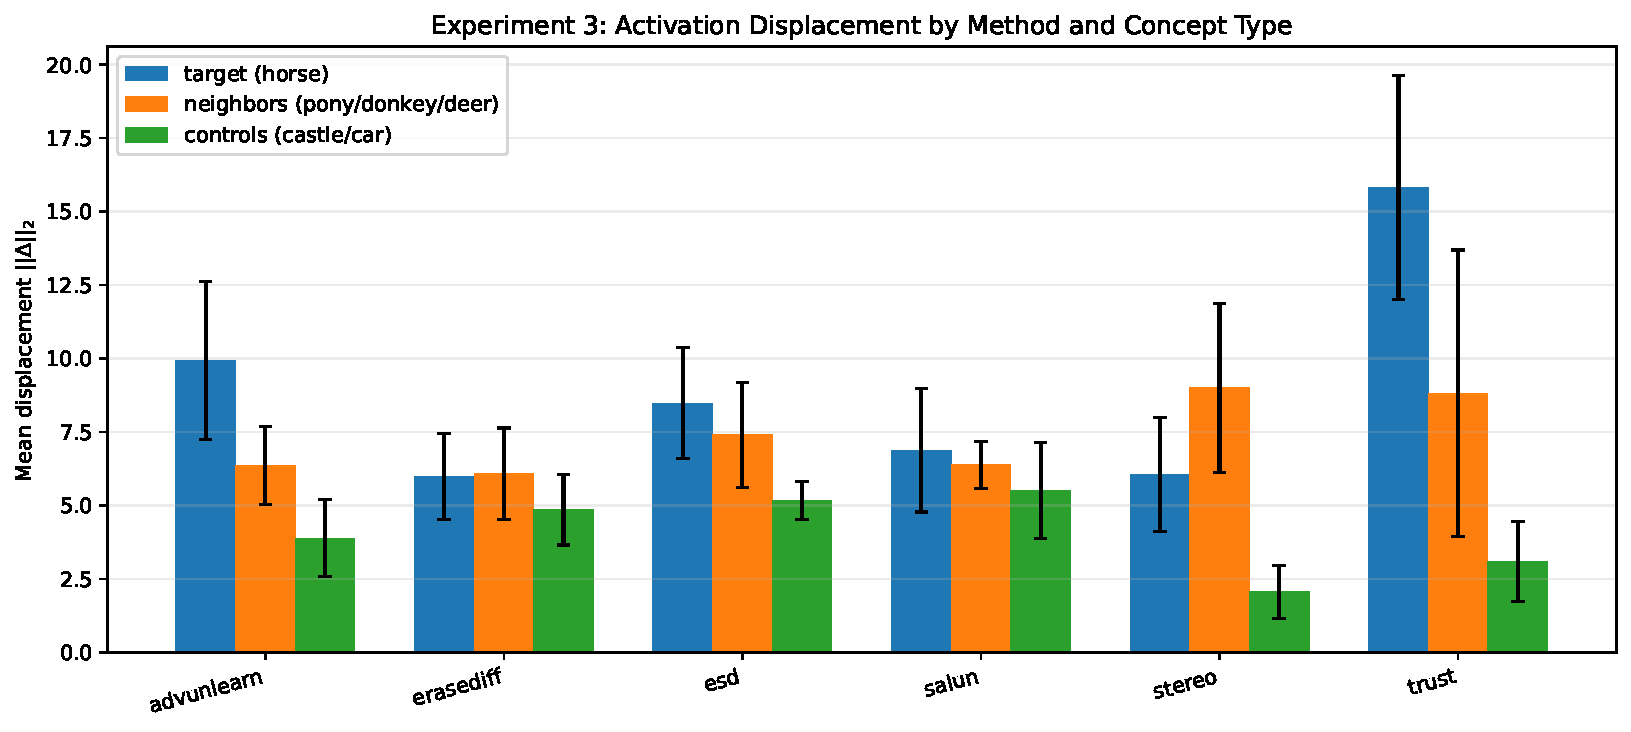
\includegraphics[width=0.8\linewidth]{img/fig_displacement_by_method_trust.pdf}
    \caption{
Mean activation displacement $\|\boldsymbol{\Phi}_{\hat\theta}(p) - \boldsymbol{\Phi}_\theta(p)\|_2$ for six unlearning methods erasing \texttt{horse}. Target prompts (blue) confirm~\cref{asm:edit}: erasure requires measurable displacement. Neighbor prompts (orange) are displaced more than control prompts (green) for all methods, consistent with the propagation mechanism in~\cref{thm:tradeoff}.
}
    \label{fig:placeholder}
\end{figure}
\newpage
\section{New Concepts}
\begin{table*}[htbp]
\centering
\caption{Results for the five additional target concepts. Original denotes the pretrained model before unlearning. All evaluation metrics are percentages. Higher UA, IRA, NP, and CP are better; lower IRR and DamageGap are better. DamageGap is the difference between control preservation (CP) and neighbor preservation (NP).}
\label{tab:new_concept_results}
\resizebox{\textwidth}{!}{
\begin{tabular}{llccccccc}
\toprule
Concept & Method & $\hat{\kappa}$ & UA (\%) $\uparrow$ & IRR (\%) $\downarrow$ & IRA (\%) $\uparrow$ & NP (\%) $\uparrow$ & CP (\%) $\uparrow$ & DamageGap (\%) $\downarrow$ \\
\midrule
Snake
& Original  & 0.37 & 9.2 & 6.0 & 31.1 & 100.0 & 100.0 & 0.0 \\
& EraseDiff & 0.37 & 88.1 & 8.6 & 19.1 & 81.2 & 93.6 & 12.4 \\
& ESD       & 0.37 & 97.9 & 6.8 & 20.6 & 81.3 & 98.1 & 16.8 \\
& SalUn     & 0.37 & 100.0 & 0.0 & 5.5 & 72.4 & 86.2 & 13.8 \\
& STEREO    & 0.37 & 100.0 & 0.0 & 14.8 & 25.1 & 96.0 & 71.1 \\
\midrule
Fish
& Original  & 0.52 & 6.2 & 11.0 & 40.5 & 100.0 & 100.0 & 0.0 \\
& EraseDiff & 0.52 & 92.3 & 5.3 & 23.2 & 78.0 & 92.1 & 14.1 \\
& ESD       & 0.52 & 94.5 & 2.7 & 34.5 & 79.2 & 98.0 & 18.8 \\
& SalUn     & 0.52 & 100.0 & 0.0 & 14.9 & 67.5 & 97.8 & 30.3 \\
& STEREO    & 0.52 & 100.0 & 0.0 & 5.8 & 23.2 & 38.4 & 15.2 \\
\midrule
Tree
& Original  & 0.63 & 4.4 & 61.8 & 51.8 & 100.0 & 100.0 & 0.0 \\
& EraseDiff & 0.63 & 32.0 & 55.2 & 53.8 & 75.1 & 98.0 & 22.9 \\
& ESD       & 0.63 & 39.7 & 48.0 & 50.3 & 82.4 & 98.9 & 16.5 \\
& SalUn     & 0.63 & 100.0 & 0.0 & 5.8 & 62.7 & 88.0 & 25.3 \\
& STEREO    & 0.63 & 100.0 & 0.0 & 4.9 & 26.6 & 32.0 & 5.4 \\
\midrule
Butterfly
& Original  & 0.66 & 7.1 & 12.2 & 36.0 & 100.0 & 100.0 & 0.0 \\
& EraseDiff & 0.66 & 46.2 & 37.3 & 34.6 & 74.7 & 92.5 & 17.8 \\
& ESD       & 0.66 & 72.6 & 28.9 & 31.2 & 78.1 & 83.3 & 5.2 \\
& SalUn     & 0.66 & 100.0 & 0.0 & 0.9 & 73.1 & 93.9 & 20.8 \\
& STEREO    & 0.66 & 100.0 & 0.0 & 10.5 & 19.2 & 68.0 & 48.8 \\
\midrule
Car
& Original  & 0.83 & 2.6 & 60.0 & 87.5 & 100.0 & 100.0 & 0.0 \\
& EraseDiff & 0.83 & 47.4 & 49.3 & 69.2 & 78.7 & 91.2 & 12.4 \\
& ESD       & 0.83 & 60.5 & 28.6 & 75.8 & 73.8 & 98.6 & 24.8 \\
& SalUn     & 0.83 & 79.3 & 16.1 & 17.8 & 66.8 & 85.6 & 18.8 \\
& STEREO    & 0.83 & 99.1 & 4.3 & 21.1 & 16.0 & 75.2 & 59.1 \\
\bottomrule
\end{tabular}
}
\end{table*}
\newpage
\section{Pareto with dashed lines}
\begin{figure}[htbp]
    \centering
    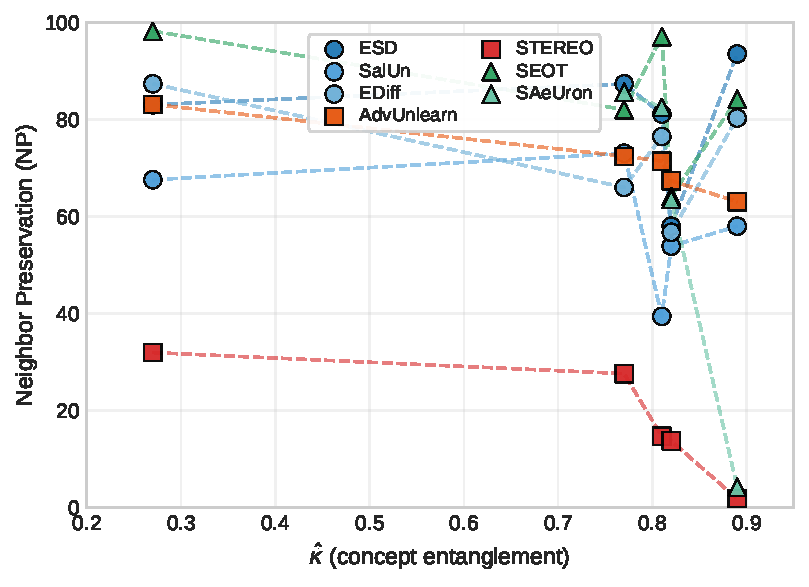
\includegraphics[width=0.5\linewidth]{img/kappa_np_scaling_dashed.pdf}
    \caption{NP across concept entanglement levels for each unlearning method. Dashed lines connect concept-specific operating points from the same method in increasing order of $\hat{\kappa}$ and are included as visual guides rather than fitted trends. Robust methods such as STEREO show a pronounced decline in NP as entanglement increases, while other methods exhibit weaker or more concept-dependent trends.}
    \label{fig:Pareto_dashed}
\end{figure}
\newpage